%<<echo=FALSE>>=
%OLD <- options(width=90)
%@
%<<echo=FALSE>>=
%options(OLD) 
%@

\documentclass{beamer}\usepackage[]{graphicx}\usepackage[]{color}
%% maxwidth is the original width if it is less than linewidth
%% otherwise use linewidth (to make sure the graphics do not exceed the margin)
\makeatletter
\def\maxwidth{ %
  \ifdim\Gin@nat@width>\linewidth
    \linewidth
  \else
    \Gin@nat@width
  \fi
}
\makeatother

\definecolor{fgcolor}{rgb}{0.102, 0.102, 0.102}
\newcommand{\hlnum}[1]{\textcolor[rgb]{0.2,0.2,0.2}{#1}}%
\newcommand{\hlstr}[1]{\textcolor[rgb]{0.2,0.2,0.2}{#1}}%
\newcommand{\hlcom}[1]{\textcolor[rgb]{0.302,0.302,0.302}{\textit{#1}}}%
\newcommand{\hlopt}[1]{\textcolor[rgb]{0.102,0.102,0.102}{#1}}%
\newcommand{\hlstd}[1]{\textcolor[rgb]{0.102,0.102,0.102}{#1}}%
\newcommand{\hlkwa}[1]{\textcolor[rgb]{0.102,0.102,0.102}{#1}}%
\newcommand{\hlkwb}[1]{\textcolor[rgb]{0.102,0.102,0.102}{#1}}%
\newcommand{\hlkwc}[1]{\textcolor[rgb]{0.2,0.2,0.2}{#1}}%
\newcommand{\hlkwd}[1]{\textcolor[rgb]{0.102,0.102,0.102}{\textbf{#1}}}%

\usepackage{framed}
\makeatletter
\newenvironment{kframe}{%
 \def\at@end@of@kframe{}%
 \ifinner\ifhmode%
  \def\at@end@of@kframe{\end{minipage}}%
  \begin{minipage}{\columnwidth}%
 \fi\fi%
 \def\FrameCommand##1{\hskip\@totalleftmargin \hskip-\fboxsep
 \colorbox{shadecolor}{##1}\hskip-\fboxsep
     % There is no \\@totalrightmargin, so:
     \hskip-\linewidth \hskip-\@totalleftmargin \hskip\columnwidth}%
 \MakeFramed {\advance\hsize-\width
   \@totalleftmargin\z@ \linewidth\hsize
   \@setminipage}}%
 {\par\unskip\endMakeFramed%
 \at@end@of@kframe}
\makeatother

\definecolor{shadecolor}{rgb}{.97, .97, .97}
\definecolor{messagecolor}{rgb}{0, 0, 0}
\definecolor{warningcolor}{rgb}{1, 0, 1}
\definecolor{errorcolor}{rgb}{1, 0, 0}
\newenvironment{knitrout}{}{} % an empty environment to be redefined in TeX

\usepackage{alltt}% regular slides (with pauses)
%\documentclass[handout]{beamer}% handout (no pauses)

%%%%%%%%%%%%%%%%%%%%%%%%%%%%%%%%%%%%%%%%%%%%%%%%%%%%%%%%%%%%%%%%%%%%%%%%%
%%%%%%% Change the lecture information here %%%%%%%%%%%%%%%%
\def\chapnum{Week \#5}
\title{STAT234: Lecture 6 - Inference methods}
\author{Kushal K. Dey}
\date{}
%%%%%%%%%%%%%%%%%%%%%%%%%%%%%%%%%%%%%%%%%%%%%%%%%%%%%%%%%%%%%%%%%%%%%%%%%

%%%%%% Start of suggested definitions and packages %%%%%%%%%%%%
%%%%%% Do not change unless you really know what you are doing %%%%%%%%%%
%%%%%%%%%%%%%%%%%%%%%%%%%%%%%%%%%%%%%%%%%%%%%%%%%%%%%%%%%%%%%%%%%%%%%%%%%

\usepackage{enumerate}
\usepackage{amsmath, bbm}
\usepackage[misc]{ifsym} % for the dice symbol \Cube{}
\usepackage[latin1]{inputenc}
\usepackage{hyperref}
\usepackage{multirow}

%\usepackage{comment}
%\usepackage{pstricks}
%\usepackage{graphicx}
%\usepackage{booktabs}
%\usepackage{pgfpages}
%\pgfpagesuselayout{2 on 1}[a4paper,border shrink=3mm]
%\pgfpagesuselayout{4 on 1}[a4paper,landscape,border shrink=3mm

\usepackage{setspace}
\ifdefined\knitrout
  \renewenvironment{knitrout}{\begin{spacing}{0.75}\begin{tiny}}{\end{tiny}\end{spacing}}
\else
\fi

%%%%%%%%%%%%%%% Defined Shortcuts (macros) %%%%%%%%%%%%%
% parameters and statistics
\newcommand{\xbar}{\overline{x}}
\newcommand{\Xbar}{\overline{X}}
\newcommand{\ybar}{\overline{y}}
\newcommand{\Ybar}{\overline{Y}}
\newcommand{\dbar}{\overline{d}}
\newcommand{\Dbar}{\overline{D}}
\newcommand{\zbar}{\overline{z}}
\newcommand{\Zbar}{\overline{Z}}
\newcommand{\ehat}{\widehat{\epsilon}}
\newcommand{\yhat}{\widehat{y}}
\newcommand{\Yhat}{\widehat{Y}}
\newcommand{\betaa}{{\beta_0}}
\newcommand{\betab}{{\beta_1}}
\newcommand{\betac}{{\beta_2}}
\newcommand{\betad}{{\beta_3}}
\newcommand{\BETA}{{\boldsymbol\beta}}
\newcommand{\betahata}{\widehat{\beta_0}}
\newcommand{\betahatb}{\widehat{\beta_1}}
\newcommand{\betahatc}{\widehat{\beta_2}}
\newcommand{\betahatd}{\widehat{\beta_3}}
\newcommand{\bhat}{\widehat{b}}
\newcommand{\btilde}{\widetilde{b}}
\newcommand{\ahat}{\widehat{a}}
\newcommand{\atilde}{\widetilde{a}}
\newcommand{\rss}{\mathit{SSE}}
\newcommand{\sigmahat}{\widehat{\sigma}}
\newcommand{\betahat}{\widehat{\beta}}
\newcommand{\thetahat}{\widehat{\theta}}
\newcommand{\phat}{\widehat{p}}
\newcommand{\pihat}{\widehat{\pi}}
\newcommand{\muhat}{\widehat{\mu}}
% real numbers and integers
\newcommand{\reals}{\mathbbm{R}}
\newcommand{\integers}{\mathbbm{N}}
%distributions
\newcommand{\normal}{\textsf{Norm}}
\newcommand{\Bin}{\textsf{Binom}}
\newcommand{\Uni}{\textsf{Unif}}
\newcommand{\Poisson}{\textsf{Pois}}
\newcommand{\Exp}{\textsf{Exp}}
\newcommand{\Beta}{\textsf{Beta}}
\newcommand{\iid}{\stackrel{\mathrm{iid}}{\sim}}
% probability and expected value
\newcommand{\rv}{r.v.\ }
\newcommand{\prob}{{\rm P}}
\newcommand{\mean}{\mathrm{E}}
\newcommand{\var}{\mathrm{Var}}
\newcommand{\Var}{\mathrm{Var}}
\newcommand{\cov}{\mathrm{Cov}}
\newcommand{\corr}{\mathop{\mathrm{Corr}}}
% measures of spread
\newcommand{\IQR}{\textit{IQR}}
\newcommand{\SAD}{\textit{SAD}}
\newcommand{\MAD}{\textit{MAD}}
\newcommand{\SSD}{\textit{SSD}}
\newcommand{\MSD}{\textit{MSD}}
\newcommand{\RMSD}{\textit{RMSD}}
\newcommand{\MSE}{\textit{MSE}}
\newcommand{\MSR}{\textit{MSR}}
% formatting code and such
\providecommand{\variable}[1]{}
\renewcommand{\variable}[1]{{\color{green!50!black}\texttt{#1}}}
\providecommand{\function}[1]{}
\renewcommand{\function}[1]{{\color{purple!75!blue}\texttt{\StrSubstitute{#1}{()}{}()}}}
\providecommand{\option}[1]{}
\renewcommand{\option}[1]{{\color{brown!80!black}\texttt{#1}}}
\providecommand{\pkg}[1]{}
\renewcommand{\pkg}[1]{{\color{red!80!black}\texttt{#1}}}
\providecommand{\code}[1]{}
\renewcommand{\code}[1]{{\color{blue!80!black}\texttt{#1}}}

%%%%%%%%%
% Changed by Kushal K Dey, University of Chicago
%\providecommand{\file}[1]{}
%\renewcommand{\file}[1]{{\tt #1}}
\providecommand{\file}[1]{}
\renewcommand{\file}[1]{{\color{orange!80!black}\texttt{#1}}}
%\providecommand{\dataframe}[1]{}
%\renewcommand{\dataframe}[1]{{\color{blue!80!black}\texttt{#1}}}
\providecommand{\dataframe}[1]{}
\renewcommand{\dataframe}[1]{{\color{cyan!80!black}\texttt{#1}}}
%%%%%%%%%

% other
\def\Sum{\sum\nolimits}
\def\b#1{\fboxsep=0pt\colorbox{black}{\color{white}\Cube{#1}}}
\def\w#1{\Cube{#1}}
%%%%%%%%%%%% End of shortcuts (macros) ##############

%%%%%%%%% One way to hide answers until you want to show them %%%%%%%%%
\def\Hide#1#2{\ul{~~~\onslide<#1>{\alert{#2}}~~~}}
\def\hide#1#2{\ul{~~\onslide<#1>{\alert{#2}}~~}}
\def\hid#1#2{\onslide<#1>{\alert{#2}}}
% Choose the color of answers here too
\setbeamercolor{alerted text}{fg=darkgray} 
%\setbeamercolor{alerted text}{fg=black} 

%------Centered Page Number Setup ------
\defbeamertemplate{footline}{centered page number}
{%
  \hspace*{\fill}%
  %\usebeamercolor[fg]{page number in head/foot}%
  %\usebeamerfont{page number in head/foot}%
  \tiny \chapnum: Page \insertframenumber\, of \inserttotalframenumber%
  \hspace*{\fill}\vskip2pt%
}
%\setbeamertemplate{footline}{\hfill\insertframenumber/\inserttotalframenumber}
\setbeamertemplate{footline}[centered page number]
%--------------------------------

%\usetheme{Copenhagen}
\setbeamertemplate{navigation symbols}{}
\usepackage[english]{babel}
\def\ul{\underline}
\linespread{1.1}
% or whatever



%\parskip=0pt
\IfFileExists{upquote.sty}{\usepackage{upquote}}{}
\begin{document}%large

%<<setup, include=FALSE, cache=FALSE>>=
%options(replace.assign=TRUE,width=90, digits=4)
%opts_chunk$set(fig.path='figure/graphics-', cache.path='cache/graphics-', fig.align='center', fig.width=8, fig.height=4.5, fig.show='as.is', out.width='0.9\\linewidth', cache=FALSE, par=TRUE, size = 'tiny', tidy=TRUE, cache.extra=rand_seed)
%knit_hooks$set(par=function(before, options, envir){
%if (before && options$fig.show!='none') par(mar=c(4,4,.1,.1),cex.lab=.95,cex.axis=.9,mgp=c(2,.7,0),tcl=-.3)
%}, document = function(x) {
%  gsub('\\\\(begin|end)\\{kframe\\}', '', x)
%}, crop=hook_pdfcrop)
%@
%<<setup2, include=FALSE, cache=FALSE>>=
%knit_theme$set("print")
%@


%%%%%%%%%%%%%%%%%%%%%%%%%%%%%%%%%%%%%%%%%%%%%%%%%%%%%%%%%%%%%%%%%%%%%%%%%
%%%%%%%%%%%%%%%%%%%%%%%%%%%%%%%%%%%%%%%%%%%%%%%%%%%%%%%%%%%%%%%%%%%%%%%%%
%%%%%% End of suggested definitions and packages %%%%%%%%%%%%

%------------------------------------------------------------------
%------------------------------------------------------------------

%%%%%%%%%% Title frame (optional) %%%%%%%%%%%%%
\begin{frame}{}
\maketitle
\end{frame}
%%%%%%%%%%%%%%%%%%%%%%%%%%%%%%%%%%%%%%%%%%%%%%%

%%%%%%%%%%%%%% Begin slides here %%%%%%%%%%%%%%

%%%%%%%%%%%%%%%%%%%%%%%%%%%%%%%%%%%%%%%%%%%%%%%
\begin{frame}{Example: Does exercise make strong bones?}
%%%%%%%%%%%%%%%%%%%%%%%%%%%%%%%%%%%%%%%%%%%%%%%

\begin{center}

\includegraphics[width=6.5cm,height=7.3 cm]{exercise.jpg}
\end{center}

\end{frame}
%%%%%%%%%%%%%%%%%%%%%%%%%%%%%%%%%%%%%%%%%%%%%%%


%%%%%%%%%%%%%%%%%%%%%%%%%%%%%%%%%%%%%%%%%%%%%%%
\begin{frame}{Example: Does exercise make strong bones?}
%%%%%%%%%%%%%%%%%%%%%%%%%%%%%%%%%%%%%%%%%%%%%%%

    Can a 6-month exercise program increase the total body bone
    mineral content (TBBMC) of young women? 
    A team of researchers is planning a study to examine this question.\\ \pause
\bigskip
    Based on the results of
    a previous study, they are willing to assume that pop. standard error $\sigma=2$ for the percent change in TBBMC over the 6-month period. Assume the sample size
     is 25.\\ \pause
    \begin{itemize}
    \item
    What are the hypotheses? \pause
    \item
    A change in TBBMC of $1\%$ change would be considered important. How to check if that is the case or not?
     \item
    What's the rejection region under $5\%$ significance level? \pause
 \end{itemize}

\end{frame}
%%%%%%%%%%%%%%%%%%%%%%%%%%%%%%%%%%%%%%%%%%%%%%%

%%%%%%%%%%%%%%%%%%%%%%%%%%%%%%%%%%%%%%%%%%%%%%%
\begin{frame}{Framing the hypothesis testing}
%%%%%%%%%%%%%%%%%%%%%%%%%%%%%%%%%%%%%%%%%%%%%%%

Let $\mu$ denote the mean percent change of the population of young women. We do not know $\mu$.  \pause \newline

We test 

$$ H_{0}: \mu = 0 \hspace{1 cm}  H_{1}: \mu > 0 $$ \pause

Assume we have $25$ values $X_1, X_2, \cdots, X_{25}$ of observed percent changes in TBBMC for $25$ women. \pause

Suppose we assume normality 

$$ X_i \sim N(\mu, \sigma^2) $$ \pause

But from previous study, we know $\sigma^2=4$. So,  \pause

$$ X_i \sim N(\mu, 4) $$ 

\end{frame}
%%%%%%%%%%%%%%%%%%%%%%%%%%%%%%%%%%%%%%%%%%%%%%%

%%%%%%%%%%%%%%%%%%%%%%%%%%%%%%%%%%%%%%%%%%%%%%%
\begin{frame}{Example: Definitions}
%%%%%%%%%%%%%%%%%%%%%%%%%%%%%%%%%%%%%%%%%%%%%%%

What is \textit{rejection region}? \pause \newline

The region such that if the data occurs in that region, we will reject the null hypothesis. \pause \newline

What is \textit{significance level}?  \pause \newline

It is a threshold for the p-value, or the probability of observing something as extreme as what you have observed from the data. If the p-value is less than this threshold, we reject.

\end{frame}
%%%%%%%%%%%%%%%%%%%%%%%%%%%%%%%%%%%%%%%%%%%%%%%


%%%%%%%%%%%%%%%%%%%%%%%%%%%%%%%%%%%%%%%%%%%%%%%
\begin{frame}{Framing the hypothesis testing}
%%%%%%%%%%%%%%%%%%%%%%%%%%%%%%%%%%%%%%%%%%%%%%%

We can write 

$$ \bar{X} \sim N(\mu, \frac{\sigma^2}{n}) $$ \pause

here 

$$ \bar{X} \sim N(\mu, \frac{4}{25}) $$ \pause

Under $H_0$ or if $H_0$ is true, we can assume $\mu_0 = 0$. Then we can write 

$$ \bar{X} \sim N(0, \frac{4}{25}) \hspace{1 cm} under \; H_0 $$ \pause

$$ \frac{\sqrt{25}}{\sqrt{4}} \bar{X} \sim N(0,1) \hspace{1 cm} under \; H_0 $$

\end{frame}
%%%%%%%%%%%%%%%%%%%%%%%%%%%%%%%%%%%%%%%%%%%%%%%


%%%%%%%%%%%%%%%%%%%%%%%%%%%%%%%%%%%%%%%%%%%%%%%
\begin{frame}{Hypothesis testing}
%%%%%%%%%%%%%%%%%%%%%%%%%%%%%%%%%%%%%%%%%%%%%%%

If we wanted to test at $5\%$ level of significance, meaning if we wanted to reject whenever p-value is less than $0.05$, then we would choose a value $c$ so that if 
we had observed $c$ as the realization of $\bar{X}$, we reject the null hypothesis.

$$ Pr_{H_0} \left [ \bar{X} > c \right ] < 0.05 $$ \pause

The left hand side is definition of p-value when $c$ is observed and for the $c$ to be an extreme value, we want that p-value to be less than 0.05. \pause \newline

Why is it one-sided here? \pause \newline

What is the smallest $c$ for which we get this property to hold. Get $c$ so that 


$$ Pr_{H_0} \left [ \bar{X} > c \right ] = 0.05 $$ \pause

\end{frame}
%%%%%%%%%%%%%%%%%%%%%%%%%%%%%%%%%%%%%%%%%%%%%%%

%%%%%%%%%%%%%%%%%%%%%%%%%%%%%%%%%%%%%%%%%%%%%%%
\begin{frame}{Hypothesis testing}
%%%%%%%%%%%%%%%%%%%%%%%%%%%%%%%%%%%%%%%%%%%%%%%

That $c$ would form the boundary between acceptance region $\bar{X} < c$, the set of all realizations for which p-value would be greater than 0.05 and we would accept null,
and the rejection region $\bar{X}> c$, the region for which we will reject the null hypothesis. \pause \newline

$$ Pr_{H_0} \left [ \bar{X} > c \right ] = 0.05 $$
$$ Pr_{H_0} \left [ \frac{\sqrt{25}}{\sqrt{4}} \bar{X} > \frac{\sqrt{25}}{\sqrt{4}} c \right ]=0.05 $$
$$ Pr_{H_0} \left [ Z > \frac{5}{2} c \right ]=0.05 $$ \pause


We know that 

$$ Pr_{H_0} \left [ Z > 1.645 \right ]=0.05 $$ \pause

\end{frame}
%%%%%%%%%%%%%%%%%%%%%%%%%%%%%%%%%%%%%%%%%%%%%%%

%%%%%%%%%%%%%%%%%%%%%%%%%%%%%%%%%%%%%%%%%%%%%%%
\begin{frame}{Hypothesis testing}
%%%%%%%%%%%%%%%%%%%%%%%%%%%%%%%%%%%%%%%%%%%%%%%

So we get 

$$ \frac{5}{2} c = 1.645 $$ \pause

implies 

$$ c = 1.645 \times \frac{2}{5} = 0.658 $$ \pause

So the rejection region under $5\%$ level of significance is $\bar{X} > 0.658$. \pause

That was all model......\pause

Now look at the data, the realization $\bar{x}$ of the random variable $\bar{X}$. \pause

\end{frame}
%%%%%%%%%%%%%%%%%%%%%%%%%%%%%%%%%%%%%%%%%%%%%%%

%%%%%%%%%%%%%%%%%%%%%%%%%%%%%%%%%%%%%%%%%%%%%%%
\begin{frame}{Hypothesis testing}
%%%%%%%%%%%%%%%%%%%%%%%%%%%%%%%%%%%%%%%%%%%%%%%

If say the observed value $\bar{x}=0.6$, then we will accept the null, meaning there is no effect of the program. \pause  \newline

If say the observed value $\bar{x}=0.9$, then we will reject the null, meaning there is a positive effect of the program. \pause \newline

The test is one-sided because as per research the alternative is that the program is effective and there is a positive change or increase in TBBMC. Thats why the alternative was $\mu > 0$. \pause

\end{frame}
%%%%%%%%%%%%%%%%%%%%%%%%%%%%%%%%%%%%%%%%%%%%%%%

%%%%%%%%%%%%%%%%%%%%%%%%%%%%%%%%%%%%%%%%%%%%%%%
\begin{frame}{Hypothesis testing}
%%%%%%%%%%%%%%%%%%%%%%%%%%%%%%%%%%%%%%%%%%%%%%%

Okay, we define some terminologies now.... \pause  \newline

\textbf{Type I error}: The probability we reject the null when the null is true. \pause

For example, if we reject when $\bar{X} > 0.658$, then under the null, $\mu=0$, we have

$$ Type \; I \; error: Pr \left [ \bar{X} > 0.658 | \mu=0 \right ] = 0.05 $$ \pause

If we reject when $\bar{X} > 0.8$, then 

$$ Type \; I \; error: Pr \left [ \bar{X} > 0.8 | \mu=0 \right ] = 0.0006 $$ \pause

As we increase $c$, we make Type I error small.

\end{frame}
%%%%%%%%%%%%%%%%%%%%%%%%%%%%%%%%%%%%%%%%%%%%%%%


%%%%%%%%%%%%%%%%%%%%%%%%%%%%%%%%%%%%%%%%%%%%%%%
\begin{frame}{Hypothesis testing}
%%%%%%%%%%%%%%%%%%%%%%%%%%%%%%%%%%%%%%%%%%%%%%%

$$ Type \; I \; error: Pr \left [ Z > \frac{\sqrt{n}}{\sigma}c | \mu=0 \right ] = 0.05  \hspace{1 cm} Z \sim N(0,1) $$ \pause

So we can reduce this Type I error by increasing $c$, but does it solve the problem? \pause \newline

Should we take $c$ to be infinity then? \pause \newline

NO....there is another error to worry about  \pause \newline

What is the probability we accept the null when the null is not true. \pause \newline

This is called the \textbf{Type II error}.

\end{frame}
%%%%%%%%%%%%%%%%%%%%%%%%%%%%%%%%%%%%%%%%%%%%%%%

%%%%%%%%%%%%%%%%%%%%%%%%%%%%%%%%%%%%%%%%%%%%%%%
\begin{frame}{Hypothesis testing}
%%%%%%%%%%%%%%%%%%%%%%%%%%%%%%%%%%%%%%%%%%%%%%%

What do you mean by null not being TRUE. What is $\mu$ then? \pause \newline

Well, $\mu > 0$, so lets fix one such $\mu$, say $\mu=1$. \pause \newline

Type II error can be written as 

$$ Type \; II \; error:  Pr \left [ \bar{X} < 0.658 | \mu=1 \right] $$ \pause \newline

Under this set up, since we know 

$$ \bar{X} \sim N(\mu=1, \frac{4}{25}) $$

\end{frame}
%%%%%%%%%%%%%%%%%%%%%%%%%%%%%%%%%%%%%%%%%%%%%%%

%%%%%%%%%%%%%%%%%%%%%%%%%%%%%%%%%%%%%%%%%%%%%%%
\begin{frame}{Hypothesis testing}
%%%%%%%%%%%%%%%%%%%%%%%%%%%%%%%%%%%%%%%%%%%%%%%

$$ Type \; II \; error:  Pr \left [ \frac{5}{2} (\bar{X} - 1) < \frac{5}{2}(0.658-1) | \mu=1 \right] $$

$$ Type \; II \; error:  Pr \left [ Z < -0.855 |\mu=1 \right ] $$

$$ Type \; II \; error:  Pr \left [ Z < -0.855  \right] \; Z \sim N(0,1) $$

This can be calculated using Normal table that Type II error is $0.1963$.


The important thing is for any  $c$ we choose as the boundary between acceptance and rejection 

$$ Type \; II \; error:  Pr \left [ Z < \frac{5}{2}(c-1)  \right] \; Z \sim N(0,1) $$

\end{frame}
%%%%%%%%%%%%%%%%%%%%%%%%%%%%%%%%%%%%%%%%%%%%%%%

%%%%%%%%%%%%%%%%%%%%%%%%%%%%%%%%%%%%%%%%%%%%%%%
\begin{frame}{Hypothesis testing}
%%%%%%%%%%%%%%%%%%%%%%%%%%%%%%%%%%%%%%%%%%%%%%%

Note that as $c$ increases, the Type II error increases. \pause \newline

So, as $c$ increases, Type I error decreases and Type II error increases \pause \newline

Statisticians use an alternative to Type II error called \textit{power}. \pause \newline

\textbf{Power}: Probability of rejecting the null when the null is not true.

What is the power when $\mu=1$?

$$ Power: Pr \left [ \bar{X} > 0.658 | \mu=1 \right] $$

\end{frame}
%%%%%%%%%%%%%%%%%%%%%%%%%%%%%%%%%%%%%%%%%%%%%%%

%%%%%%%%%%%%%%%%%%%%%%%%%%%%%%%%%%%%%%%%%%%%%%%
\begin{frame}{Hypothesis testing}
%%%%%%%%%%%%%%%%%%%%%%%%%%%%%%%%%%%%%%%%%%%%%%%

$$ Power:  Pr \left [ Z > \frac{\sqrt{n}}{\sigma}(c-1)  \right] \; Z \sim N(0,1) $$

where $\sigma=2$ and $n=25$.

So power decreases  as $c$ increases. \pause \newline

So, as $c$ increase Type I error and power increase, the latter implying Type II error decreases because 

$$ Power : = 1 - Type \; II \; error $$

\end{frame}
%%%%%%%%%%%%%%%%%%%%%%%%%%%%%%%%%%%%%%%%%%%%%%%

%%%%%%%%%%%%%%%%%%%%%%%%%%%%%%%%%%%%%%%%%%%%%%%
\begin{frame}{Ways to Increase the Power}
%%%%%%%%%%%%%%%%%%%%%%%%%%%%%%%%%%%%%%%%%%%%%%%

  \begin{itemize}
  \item Increase $\alpha$. A $5\%$ test of significance will have a
    greater chance of rejecting the null than a $1\%$ test
    because the strength of evidence required for rejection is less. \pause

  \item Consider a particular alternative that is farther away from
    $\mu_0=0$. Values of $\mu$ that are in $H_a$ but lie close to the
     hypothesized value $\mu_0$ are harder to detect than values of
    $\mu$ that are far from $\mu_0$. \pause

  \item Increase the sample size. More data will provide more
    information about $\bar{x}$ so we have a better chance of
    distinguishing values of $\mu$. \pause

  \item Decrease $\sigma$. This has the same effect as increasing the
    sample size: it provides more information about $\mu$. Improving
    the measurement process and restricting attention to a
    subpopulation are two common ways to decrease $\sigma$. 
  \end{itemize}

\end{frame}
%%%%%%%%%%%%%%%%%%%%%%%%%%%%%%%%%%%%%%%%%%%%%%%

%%%%%%%%%%%%%%%%%%%%%%%%%%%%%%%%%%%%%%%%%%%%%%%
\begin{frame}{Example: Does exercise make strong bones? (cont.)}
%%%%%%%%%%%%%%%%%%%%%%%%%%%%%%%%%%%%%%%%%%%%%%%

\begin{small}
    \begin{itemize}

    \item Change the significance level to $\alpha =0.01 $. \pause

      The z test rejects $H_0$ at the $\alpha =0.01$ level whenever
      \[ z = \frac{ \bar{x} - \mu_0}{\sigma/\sqrt{n}}
      =\frac{\bar{x}}{2/\sqrt{25}}\geq 2.32 \] that is, we reject
      $H_0$ when $\bar{x} \geq 2.32 \frac{2}{\sqrt{25}} = 0.928$ \pause

      The power of the test at alternative $\mu= 1 $ is
      \begin{align*}
        P( \bar{x} \geq 0.928 | \mu = 1)
        &= P(\frac{\bar{x} - \mu}{\sigma/\sqrt{n}} \geq
        \frac{0.928 -1}{2/\sqrt{25}} | \mu=1)\\
        &= P(Z \geq -0.18)= 0.57
      \end{align*} \pause

    \item Change the alternative to $\mu=2$. \pause  The power of the test at alternative $\mu= 2 $ at $\alpha
      =0.01$ level is
      \begin{eqnarray*}
        P( \bar{x} \geq 0.928 | \mu = 2)
        &=& P(\frac{\bar{x} - \mu}{\sigma/\sqrt{n}} \geq
        \frac{0.928 -2}{2/\sqrt{25}} | \mu =2)\\
        &=& P(Z \geq -2.68)=0.996
      \end{eqnarray*}
      
      \end{itemize}
      \end{small}
\end{frame}
%%%%%%%%%%%%%%%%%%%%%%%%%%%%%%%%%%%%%%%%%%%%%%%

%%%%%%%%%%%%%%%%%%%%%%%%%%%%%%%%%%%%%%%%%%%%%%%
\begin{frame}{Example: Does exercise make strong bones? (cont.)}
%%%%%%%%%%%%%%%%%%%%%%%%%%%%%%%%%%%%%%%%%%%%%%%

\begin{itemize}
    \item Increase the sample size $n= 100$. \pause

      The z test rejects $H_0$ at the $\alpha =0.01$ level whenever
      \[ z=\frac{ \bar{x} - \mu_0}{\sigma/\sqrt{n}} =
      \frac{\bar{x}}{2/\sqrt{100}}\geq 2.32 \] that is, we reject
      $H_0$ when $\bar{x} \geq 2.32 \frac{2}{\sqrt{100}} = 0.464$ \pause

      The power of the test at alternative $\mu= 1 $ is
      \begin{align*}
        P(\bar{x} \geq 0.464 | \mu = 1)
        &= P(\frac{\bar{x} - \mu}{\sigma/\sqrt{n}} \geq
        \frac{0.464 -1}{2/\sqrt{100} }~| ~ \mu =1)\\
        &= P( Z \geq -2.68)= 0.996
      \end{align*}

\end{itemize}
\end{frame}
%%%%%%%%%%%%%%%%%%%%%%%%%%%%%%%%%%%%%%%%%%%%%%%

%%%%%%%%%%%%%%%%%%%%%%%%%%%%%%%%%%%%%%%%%%%%%%%
\begin{frame}{Example: Does exercise make strong bones? (cont.)}
%%%%%%%%%%%%%%%%%%%%%%%%%%%%%%%%%%%%%%%%%%%%%%%

\begin{itemize}
    \item Decrease $\sigma =1$ \pause

      The z test rejects $H_0$ at the $\alpha =0.01$ level whenever
      \[ z=\frac{ \bar{x} - \mu_0}{\sigma/\sqrt{n}} =
      \frac{\bar{x}}{1/\sqrt{100}}\geq 2.32 \] that is, we reject
      $H_0$ when $\bar{x} \geq 2.32 \frac{1}{\sqrt{100}} = 0.232$
\pause
      The power of the test at alternative $\mu= 1 $ is
      \begin{align*}
        P( \bar{x} \geq 0.232 | \mu = 1)
        &= P(\frac{\bar{x} - \mu}{\sigma/\sqrt{n}} \geq
        \frac{0.232 -1}{1/\sqrt{100}} | \mu =1) \\
 &= P( Z \geq -7.68) \approx 1
      \end{align*}

    \end{itemize}
\end{frame}
%%%%%%%%%%%%%%%%%%%%%%%%%%%%%%%%%%%%%%%%%%%%%%%

%%%%%%%%%%%%%%%%%%%%%%%%%%%%%%%%%%%%%%%%%%%%%%%
\begin{frame}{Two Types of Errors Revisited}
%%%%%%%%%%%%%%%%%%%%%%%%%%%%%%%%%%%%%%%%%%%%%%%

%  \begin{small}
    Recall that the following four outcomes are possible when conducting
    a test:

    \begin{center}
      \begin{tabular}{|c|c|c|}
        \hline
        \multirow{2}{*}{Reality} & \multicolumn{2}{c|}{Our Decision}\\
        & \multicolumn{1}{c}{$H_0$} & $H_a$\\
        \hline
        \multirow{2}{*}{$H_0$} & $\surd$ & Type I Error\\
        & ($\mbox{Prob}=1-\alpha$) & ($\mbox{Prob}=\alpha$)\\
        \cline{2-3}
        \multirow{2}{*}{$H_a$} & Type II Error & $\surd$\\
        & ($\mbox{Prob}=\beta$) & ($\mbox{Prob}=1-\beta$)\\
        \hline
      \end{tabular}
    \end{center}
\pause
    Type I error is generally {\bf more serious} than type II error. \\ \pause
    For example: $H_0:$ the person is not guilty, $H_1:$ the person is guilty\\ \pause
    Type I error \pause = convicting an innocent person\\ \pause
    Type II error \pause = failing to convict a guilty person\\ \pause  
\medskip
    In practice, we first choose an $\alpha$ and consider only tests
    with probability of Type I error no greater than $\alpha$. \pause Then we select one that makes the probability
    of Type II error as small as possible (test with most power). \pause
%  \end{small}

\end{frame}
%%%%%%%%%%%%%%%%%%%%%%%%%%%%%%%%%%%%%%%%%%%%%%%

% %%%%%%%%%%%%%%%%%%%%%%%%%%%%%%%%%%%%%%%%%%%%%%%
% \begin{frame}{Why can't we minimize both the errors?}
% %%%%%%%%%%%%%%%%%%%%%%%%%%%%%%%%%%%%%%%%%%%%%%%
% 
% \begin{itemize}
% \item $H_0:\mu=0$ vs $H_1: \mu \neq 0$. Assume $n=9, \sigma=10$ \pause
% \item We reject $H_0$ at $\alpha$ \% significance level if $|\frac{\bar{x}-0}{\sigma/\sqrt{n}}|>1.96$ \pause
% \item This gives us the rejection rule: \\ Reject $H_0$ at $\alpha$ \% significance level if $|\bar{x}| >z_{\alpha/2}\frac{\sigma}{\sqrt{n}}= z_{\alpha/2}\frac{10}{\sqrt{9}}$ \pause
% \item Now suppose the true value of $\mu$ is 2, then the $\bar{x}$ has the true distribution as Normal distribution with mean 1 and sd $\frac{\sigma}{\sqrt{n}}=\frac{10}{3}$. \pause 
% \item Using the 68-95-99.7 rule, we see that, as we decrease our $\alpha$ ( Type-1 error ) the chance that a $\bar{x}$ from a different population ( diferent from the hypothesized one ) will fall within the acceptance region of the test increases. \pause
% \item Moral: If we decrease type-I error, in general type-II error increases.
% \end{itemize}
% 
% \end{frame}
% %%%%%%%%%%%%%%%%%%%%%%%%%%%%%%%%%%%%%%%%%%%%%%%

%%%%%%%%%%%%%%%%%%%%%%%%%%%%%%%%%%%%%%%%%%%%%%%
\begin{frame}
%%%%%%%%%%%%%%%%%%%%%%%%%%%%%%%%%%%%%%%%%%%%%%%

\begin{center}
\huge{Another important continuous distribution }
\end{center}
\end{frame}
%%%%%%%%%%%%%%%%%%%%%%%%%%%%%%%%%%%%%%%%%%%%%%%

%%%%%%%%%%%%%%%%%%%%%%%%%%%%%%%%%%%%%%%%%%%%%%%
\begin{frame}{Chi-Square Distribution}
%%%%%%%%%%%%%%%%%%%%%%%%%%%%%%%%%%%%%%%%%%%%%%%

The chi-square distributions: $\chi_k^2$
$$f(x) = \frac{ x^{(k/2)-1} e^{- x/2}}{2^{k/2}\Gamma(k/2)}
  \qquad x>0,\, k\geq 1$$ \pause
$$E(X) = k \qquad Var(X) = 2k$$ \pause

\begin{center}
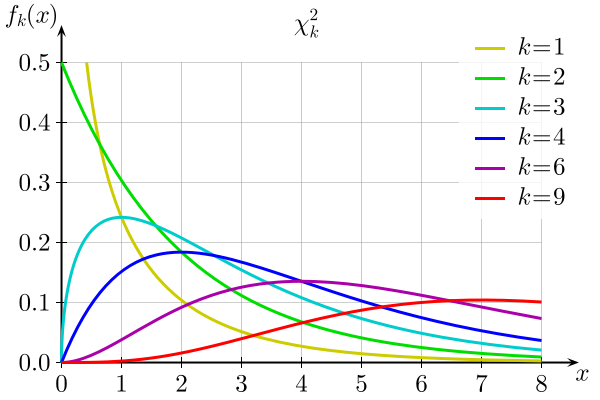
\includegraphics[width=8cm,height=4cm]{chi-square}
\end{center}


\end{frame}
%%%%%%%%%%%%%%%%%%%%%%%%%%%%%%%%%%%%%%%%%%%%%%%

%%%%%%%%%%%%%%%%%%%%%%%%%%%%%%%%%%%%%%%%%%%%%%%
\begin{frame}{Chi-Square Distribution}
%%%%%%%%%%%%%%%%%%%%%%%%%%%%%%%%%%%%%%%%%%%%%%%

The chi-square distributions: $\chi_1^2$
$$f(x) = \frac{ x^{-1/2} e^{- x/2}}{\sqrt{2\pi}}
  \qquad x>0$$ \pause
  
Origin of the Chi-square distribution: \\
Let $Z\sim N(0,1)$ and define $Y=Z^2.$  Then, $Y\sim \chi^2_1.$ \pause
\bigskip



\bigskip
In general, $\chi_n^2$ is a sum of $n$ i.i.d. standard normal distributions.

  \end{frame}
%%%%%%%%%%%%%%%%%%%%%%%%%%%%%%%%%%%%%%%%%%%%%%%

%%%%%%%%%%%%%%%%%%%%%%%%%%%%%%%%%%%%%%%%%%%%%%%
\begin{frame}{Chi-Square Distribution}
%%%%%%%%%%%%%%%%%%%%%%%%%%%%%%%%%%%%%%%%%%%%%%%

Properties:
\begin{itemize}
\item
We will need the {\bf reproductive property of $\chi^2$:}\\ \pause
Let $X_1\sim\chi^2_{n_1}, X_2\sim\chi^2_{n_2}, \ldots,
X_k\sim\chi^2_{n_k}$
with $X_1, X_2,\ldots,X_k$ independent random variables.
Define $Y=X_1+X_2+\cdots+X_k.$
Then, $Y\sim\chi^2_n$ where $n=n_1+n_2+\cdots+n_k.$ \pause
\item
Conversely, $X_1\sim\chi^2_{n_1}, X_1 + X_2\sim\chi^2_{n_1 + n_2} \Rightarrow X_2\sim\chi^2_{n_2}$. \pause 
\item
If $X_i \sim N()$, then $\bar{X}$ and $S^2$ are independent. \\ \pause
Reason: $Cov(\bar{X}, X_i - \bar{X}) = 0 \Rightarrow \bar{X}$ and $X_i - \bar{X}$ are uncorrelated\\
$\Rightarrow \bar{X}$ and  $X_i - \bar{X}$ are independent. 

\end{itemize}

\end{frame}
%%%%%%%%%%%%%%%%%%%%%%%%%%%%%%%%%%%%%%%%%%%%%%%

%%%%%%%%%%%%%%%%%%%%%%%%%%%%%%%%%%%%%%%%%%%%%%%
\begin{frame}{Chi-Square Distribution}
%%%%%%%%%%%%%%%%%%%%%%%%%%%%%%%%%%%%%%%%%%%%%%%

To get started, consider a random sample $X_1, X_2,\ldots,X_n$\\
 from a $N(\mu,\sigma^2)$ population. \pause
Let $$Z_i = \frac{X_i-\mu}{\sigma} \qquad\mbox{so that}\qquad
Z_i^2\sim\chi^2_1 \quad\mbox{and\ } Z_i's \mbox{\ are independent.}$$ \pause
Then, 
$$\sum_{i=1}^n \left[\frac{X_i-\mu}{\sigma}\right]^2 
  = \sum_{i=1}^n Z_i^2 = \sum_{i=1}^n \chi^2_1 = \chi^2_n.$$ \pause


$$\frac{(n-1)S^2}{\sigma^2}\sim\chi^2_{(n-1)}$$

\end{frame}
%%%%%%%%%%%%%%%%%%%%%%%%%%%%%%%%%%%%%%%%%%%%%%%

%%%%%%%%%%%%%%%%%%%%%%%%%%%%%%%%%%%%%%%%%%%%%%%
\begin{frame}{Mean of Sampling Distribution of $s^2$}
%%%%%%%%%%%%%%%%%%%%%%%%%%%%%%%%%%%%%%%%%%%%%%%

Since we have,
$$\frac{(n-1)S^2}{\sigma^2}\sim\chi^2_{(n-1)}$$ for a random sample from a
$N(\mu,\sigma^2)$ population, we have that
$$E\left[\frac{(n-1)S^2}{\sigma^2}\right] 
= E(\chi^2_{(n-1)}) = n-1$$ \pause
It follows that, $$n-1 = E\left[\frac{(n-1)S^2}{\sigma^2}\right]
          = \frac{(n-1)}{\sigma^2}E(S^2) \Rightarrow
E(s^2)=\sigma^2.$$

So, when sampling from a normal population, \\
$s^2$ is on target $(\sigma^2)$ on average.
\bigskip



\end{frame}
%%%%%%%%%%%%%%%%%%%%%%%%%%%%%%%%%%%%%%%%%%%%%%%

%%%%%%%%%%%%%%%%%%%%%%%%%%%%%%%%%%%%%%%%%%%%%%%
\begin{frame}{Mean of Sampling Distribution of $s^2$}
%%%%%%%%%%%%%%%%%%%%%%%%%%%%%%%%%%%%%%%%%%%%%%%

What is the mean of the sampling distribution for $S^2$ for 
samples from {\em any} population? \pause
\bigskip

First, show that $\displaystyle E \left[\sum_{i=1}^n
(X_i-\bar{X})^2\right] = (n-1)\sigma^2$\\ \pause
\bigskip
Then, we can conclude that 
$$E(S^2) = E\left[\frac{1}{n-1}\sum_{i=1}^n (X_i-\bar{X})^2\right]
= \sigma^2$$
for samples from {\em any} population. \pause
\bigskip

This is one reason why sample variance is defined by dividing by $n-1$
instead of $n.$  If we divide by $n,$ the resulting sample variance will
tend to underestimate $\sigma^2$ on average. \pause

\end{frame}
%%%%%%%%%%%%%%%%%%%%%%%%%%%%%%%%%%%%%%%%%%%%%%%

%%%%%%%%%%%%%%%%%%%%%%%%%%%%%%%%%%%%%%%%%%%%%%%
\begin{frame}{The ``Student's" $T$ Probability Distribution}
%%%%%%%%%%%%%%%%%%%%%%%%%%%%%%%%%%%%%%%%%%%%%%%

Let $Z\sim N(0,1)$ and $Y\sim\chi^2_\nu$ with $Z,Y$ {\bf independent}.
Then, $T=\frac{Z}{\sqrt{Y/\nu}}$
is said to have the $T-$distribution with $\nu$ degrees of freedom (df):
$T\sim t_n.$ \pause
\medskip
p.d.f:
$$f(t) = \frac{\Gamma(\frac{\nu+1}{2})}{\sqrt{\pi \nu} \Gamma(\frac{\nu}{2})} (1+\frac{t^2}{\nu})^{-\frac{\nu+1}{2}}, -\infty < t < \infty$$ \pause
It can be shown that $E(T) = 0$ and $Var(T) = \nu/(\nu-2).\ \nu>2$ \pause

\begin{center}
\vskip-0.6cm
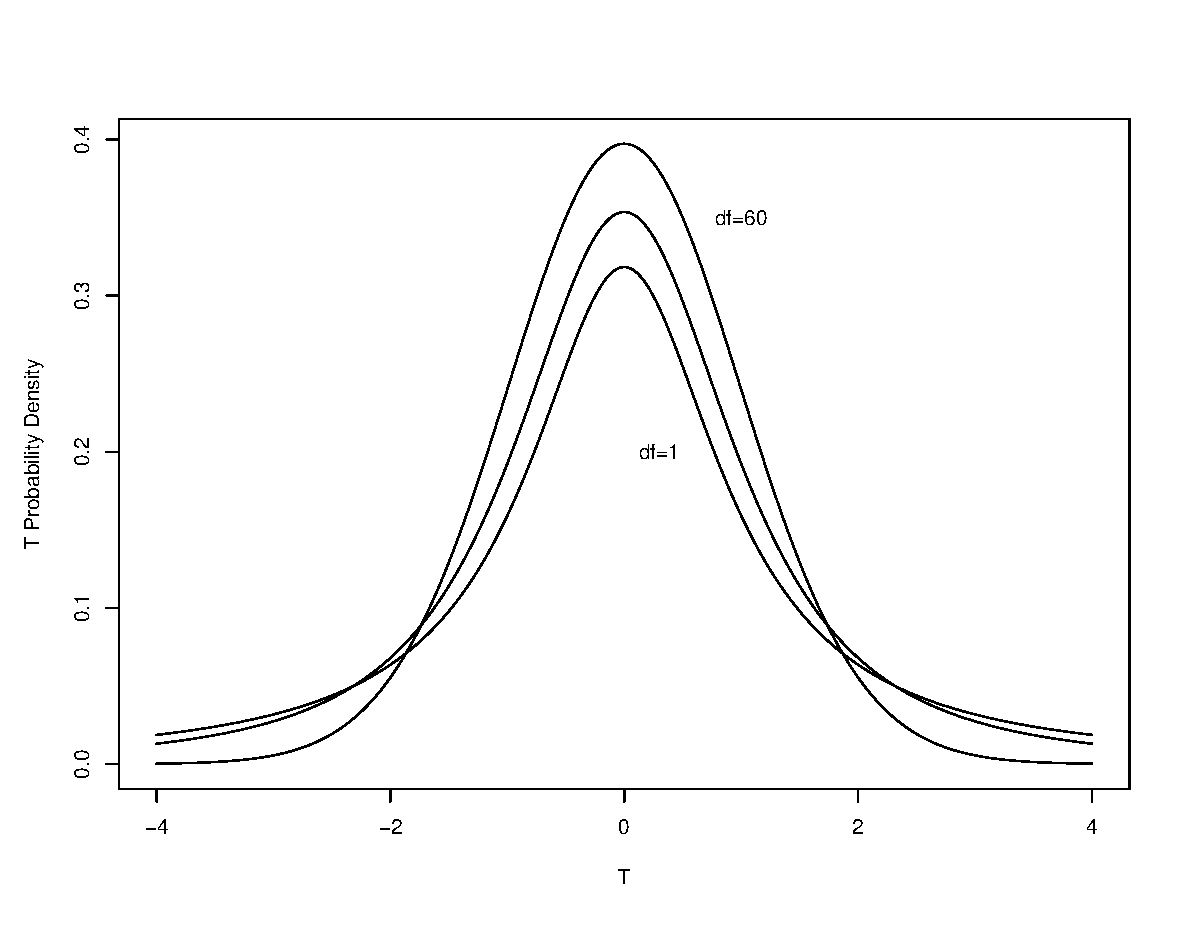
\includegraphics[width=5.5cm,height=3.5cm]{6tdistns}
\vskip-1cm
\end{center}
%> post()
%> plot(c(-400:400)/100, dt(c(-400:400)/100,
%> 1),type="l",ylim=c(0,dt(0,60)),xlab="T",ylab="T Probability Density")
%> lines(c(-400:400)/100,dt(c(-400:400)/100,60))
%> lines(c(-400:400)/100,dt(c(-400:400)/100,2))
%> text(.3,.2,labels="df=1")
%> text(1,.35,labels="df=60")
%> dev.off()
\vskip -0.6cm
\pause
{\bf Question:} What's the T distribution when $\nu \to \infty$?
\end{frame}
%%%%%%%%%%%%%%%%%%%%%%%%%%%%%%%%%%%%%%%%%%%%%%%

%%%%%%%%%%%%%%%%%%%%%%%%%%%%%%%%%%%%%%%%%%%%%%%
\begin{frame}{How is the $T-$distribution Related to Estimation?}
%%%%%%%%%%%%%%%%%%%%%%%%%%%%%%%%%%%%%%%%%%%%%%%

Let $X_1,X_2,\ldots,X_n$ be a random sample 
from a $N(\mu,\sigma^2)$ popn.
\medskip

We know that $\displaystyle Z=\frac{\bar{X}-\mu}{\sigma/\sqrt{n}}\sim N(0,1).$ \pause
\medskip

But what if $\sigma^2$ is not known? \pause
Use $s\approx\sigma$ to estimate it.
\bigskip

Consider
\begin{align*}
T &= \frac{\bar{X}-\mu}{s/\sqrt{n}} 
= \frac{\bar{X}-\mu}{\sigma/\sqrt{n}} \cdot \frac{\sigma}{s}
= Z \frac{\sigma}{s} \quad
 (\mbox{where\ } Z\sim N(0,1) )\\
&= \frac{Z}{s/\sigma} = \frac{Z}{\sqrt{s^2/\sigma^2}}\\
&= \frac{Z}{\sqrt{\frac{(n-1)s^2}{\sigma^2(n-1)}}}
 = \frac{Z}{\sqrt{\chi^2_{(n-1)}/(n-1)}}
\sim t_{(n-1)}
\end{align*}
\pause

\end{frame}
%%%%%%%%%%%%%%%%%%%%%%%%%%%%%%%%%%%%%%%%%%%%%%%

%%%%%%%%%%%%%%%%%%%%%%%%%%%%%%%%%%%%%%%%%%%%%%%
\begin{frame}{How is the $T-$distribution Related to Estimation?}
%%%%%%%%%%%%%%%%%%%%%%%%%%%%%%%%%%%%%%%%%%%%%%%

$T = \frac{\bar{X}-\mu}{s/\sqrt{n}} \sim t_{(n-1)}$ \pause

\bigskip

So, even when the popn variance $\sigma^2$ is not known, we can
still find probabilities for the sample mean $\bar{X}$ for data from a
normal popn. \pause  
\medskip

We just replace $\sigma$ by its estimate $(s)$ in the standardization of
$\bar{X}$ and then look up probabilities from the $t_{(n-1)}$ distribution
instead of the $N(0,1)$ distribution. \pause
\bigskip

The $t_{(n-1)}$ distribution is similar to the $N(0,1),$ but with more
spread (to account for the extra uncertainty in the estimate of $\sigma$.)
\medskip \pause

As sample size increases, $s$ gets closer to $\sigma$ \\
and the $t_{(n-1)}$ distribution gets closer to $N(0,1).$ \pause

\end{frame}
%%%%%%%%%%%%%%%%%%%%%%%%%%%%%%%%%%%%%%%%%%%%%%%

%%%%%%%%%%%%%%%%%%%%%%%%%%%%%%%%%%%%%%%%%%%%%%%
\begin{frame}{t-tests}
%%%%%%%%%%%%%%%%%%%%%%%%%%%%%%%%%%%%%%%%%%%%%%%

\begin{itemize}
\item Remember we discussed about the case $\sigma$ not known very briefly? \pause
\item $H_0: \mu= \mu_0$ vs $H_1: \mu_0 \neq \mu_0$. Assume $\sigma$ is known.
\item $z=\frac{\bar{x}-\mu_0}{\sigma/\sqrt{n}}$ ..\pause  $z$-test \pause
\item We reject $H_0$ if $|z|>z^*=z_{\alpha/2}$ \pause
\item If not known, replace $\sigma$ by $\hat{\sigma}=s$ \pause
\item $t=\frac{\bar{x}-\mu_0}{s/\sqrt{n}}$\pause..  $t$-test \pause
\item If $H_0$ is true, observed value $t$ follows \textit{t}- distribution with degrees of freedom $n-1$ \pause
\item We reject $H_0$ if $|t|>t_{(n-1)}^*=t_{(n-1),\alpha/2}$
\end{itemize}
\end{frame}
%%%%%%%%%%%%%%%%%%%%%%%%%%%%%%%%%%%%%%%%%%%%%%%

%%%%%%%%%%%%%%%%%%%%%%%%%%%%%%%%%%%%%%%%%%%%%%%
\begin{frame}{Example: Mouse tumor experiment}
%%%%%%%%%%%%%%%%%%%%%%%%%%%%%%%%%%%%%%%%%%%%%%%

\begin{center}
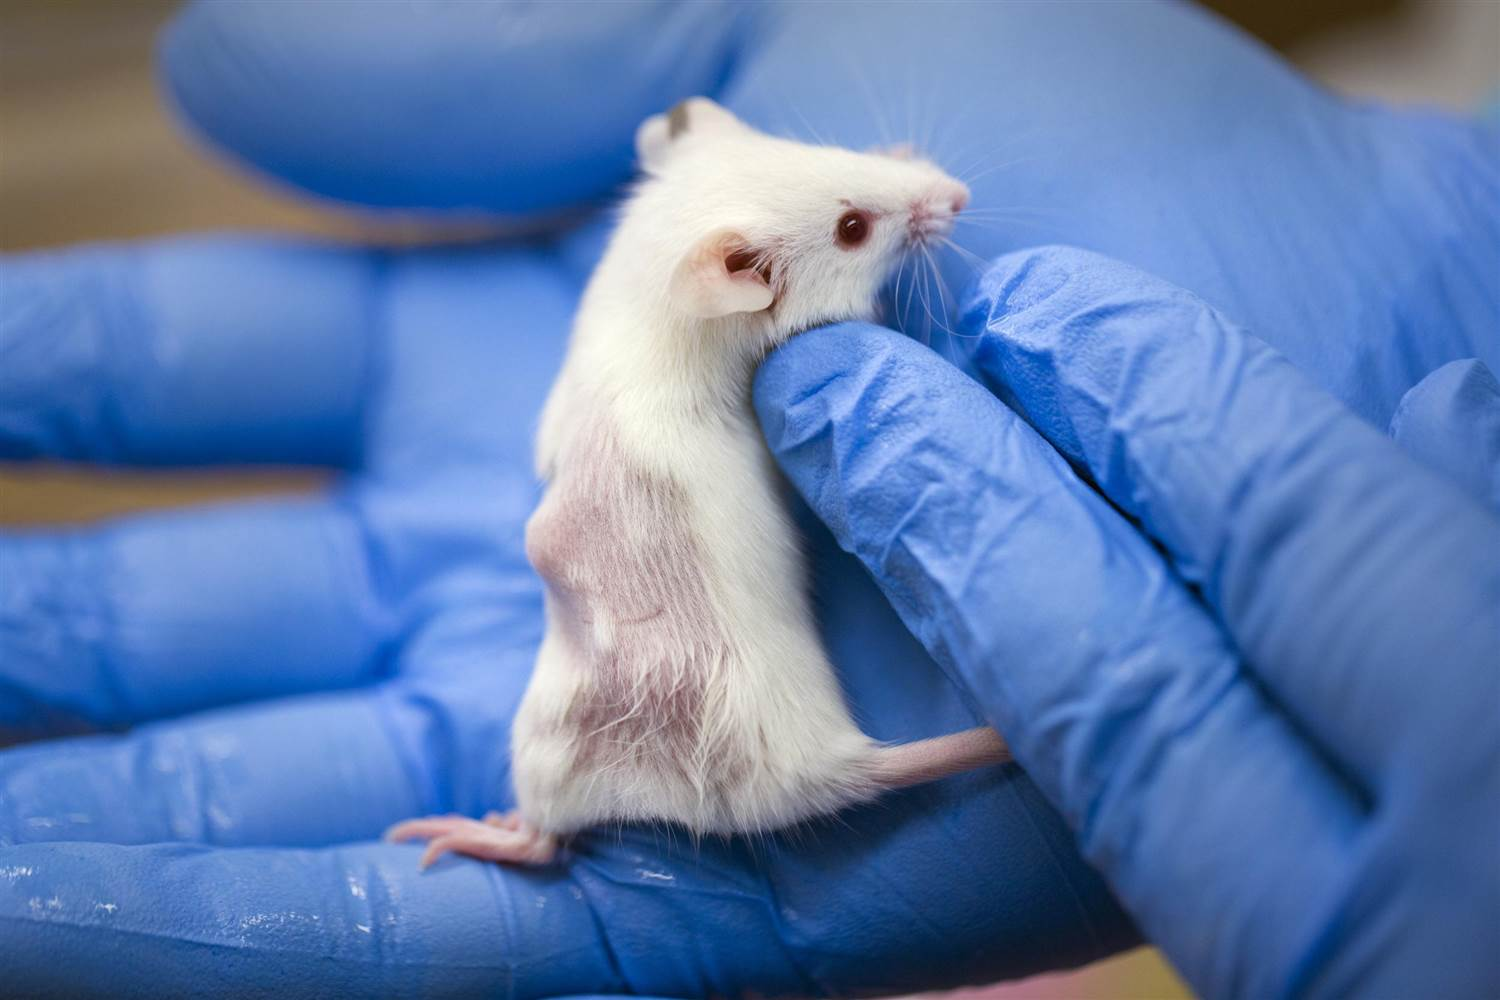
\includegraphics[width=7cm,height=5.3 cm]{mouse-tumor.jpg}
\end{center}

\end{frame}
%%%%%%%%%%%%%%%%%%%%%%%%%%%%%%%%%%%%%%%%%%%%%%%


%%%%%%%%%%%%%%%%%%%%%%%%%%%%%%%%%%%%%%%%%%%%%%%
\begin{frame}{Example: Growth of Tumor}
%%%%%%%%%%%%%%%%%%%%%%%%%%%%%%%%%%%%%%%%%%%%%%%

    Let X (in $mm$) denote the growth in 15 days of a tumor induced in
    a mouse. It is known from a previous experiment that the average
    tumor growth is $4mm$.\\ \pause
\bigskip
    A sample of 20 mice that have a genetic
    variant hypothesized to be involved in tumor growth yielded
    $\bar{x} = 3.8mm, s = 0.3mm$.\\ \pause
\bigskip
    Test whether $\mu = 4$ or not,
    assuming growths are normally distributed.

\end{frame}
%%%%%%%%%%%%%%%%%%%%%%%%%%%%%%%%%%%%%%%%%%%%%%%

%%%%%%%%%%%%%%%%%%%%%%%%%%%%%%%%%%%%%%%%%%%%%%%
\begin{frame}{Example: Growth of Tumor (Cont.)}
%%%%%%%%%%%%%%%%%%%%%%%%%%%%%%%%%%%%%%%%%%%%%%%

\footnotesize
\begin{enumerate}
    \item State the hypotheses 
      \[H_0: \mu = 4 \mbox \qquad H_a: \mu \ne 4 \] \pause
    \item Calculate the t-statistic
      \[ t = \frac{3.8-4.0}{0.3/\sqrt{20}} = -2.98 \] \pause
    \item Determine the $p$-value
      \[ p = \mbox{P}(t_{19} \ge 2.98) +  \mbox{P}(t_{19} \le -2.98) = 0.008 \] \pause
    \end{enumerate}
    Since $p$ is less than 0.01, we reject $H_0$ at significance level
    $\alpha = 0.01$. There is evidence that the population mean growth
    is not $4mm$. \pause

    What if we wanted a 99\% CI for $\mu$ instead? The CI is given by
    \begin{eqnarray*}
      \left(\bar{x} - t^{*}\frac{s}{\sqrt{n}},\;
        \bar{x} + t^{*}\frac{s}{\sqrt{n}}\right) &=& \left(3.8 - 2.861 \times \frac{0.3}{\sqrt{20}},\;
        3.8 + 2.861 \times \frac{0.3}{\sqrt{20}}\right)\\
      &=& \left(3.61,\; 3.99\right)
    \end{eqnarray*}
    where $t^{*}=t_{19,.005}=2.861$ \pause

    Note that 4 is outside this CI. From this, we can draw the same
    conclusion as from the test. Namely, at significance level
    $\alpha=0.01$, the mean growth not equal to $4mm$.
\normalsize
\end{frame}
%%%%%%%%%%%%%%%%%%%%%%%%%%%%%%%%%%%%%%%%%%%%%%%

%%%%%%%%%%%%%%%%%%%%%%%%%%%%%%%%%%%%%%%%%%%%%%%
\begin{frame}{Confidence intervals for t distribution }
%%%%%%%%%%%%%%%%%%%%%%%%%%%%%%%%%%%%%%%%%%%%%%%

$$(\bar{x}-t^* \frac{s}{\sqrt{n}}, \bar{x}+t^* \frac{s}{\sqrt{n}})$$ is the confidence interval for a two-sided hypothesis. If the population is normal then this is exact, otherwise it is approximate.  \pause

\begin{itemize}
\item $\sigma$ is known, $$(\bar{x}-z^* \frac{\sigma}{\sqrt{n}}, \bar{x}+z^* \frac{\sigma}{\sqrt{n}})$$ \pause
\item $\sigma$ is not known but we still use $z^*$, $$(\bar{x}-z^* \frac{s}{\sqrt{n}}, \bar{x}+z^* \frac{s}{\sqrt{n}})$$ \pause
\item $$(\bar{x}-t^* \frac{s}{\sqrt{n}}, \bar{x}+t^* \frac{s}{\sqrt{n}})$$ \pause
\end{itemize}
\vspace{-0.1 in}
\begin{center}
\url{http://www.rossmanchance.com/applets/ConfSim.html}
\end{center}
\end{frame}
%%%%%%%%%%%%%%%%%%%%%%%%%%%%%%%%%%%%%%%%%%%%%%%

%%%%%%%%%%%%%%%%%%%%%%%%%%%%%%%%%%%%%%%%%%%%%%%
\begin{frame}{Power of a t-test}
%%%%%%%%%%%%%%%%%%%%%%%%%%%%%%%%%%%%%%%%%%%%%%%

\begin{itemize}
\item $H_0: \mu=0$ vs $H_1: \mu \neq 0$ \pause
\item Find the rejection rule based on $\bar{x}$ and $s$ \pause
\item Decide on a specific alternative where you want to compute the power . Say $\mu=1$ \pause
\item Find $P( \text{Rejection rule} | \mu=1)$. Difficulty? \pause
\item Assume $s$ to be the true value of $\sigma$ and use normal probabilities to get the \textit{approximate} power.
\end{itemize}
\end{frame}
%%%%%%%%%%%%%%%%%%%%%%%%%%%%%%%%%%%%%%%%%%%%%%%

%%%%%%%%%%%%%%%%%%%%%%%%%%%%%%%%%%%%%%%%%%%%%%%
\begin{frame}{When to use a $t$- test}
%%%%%%%%%%%%%%%%%%%%%%%%%%%%%%%%%%%%%%%%%%%%%%%

\begin{itemize}
\item  \textbf{Robust:} An inference procedure is called robust if the required probability calculations are insenssitive to violations of the assumptions made. \pause
\item $t$ involves $\bar{x}$ and $s$ which are not robust to presence of outliers. So, t-test is \textit{not} robust in the presence of outlier \pause
\item  If $n>40$ then safely use t- test even if skewed \pause
\item If $15<n<40$ and no outliers or strong skewness ..use t \pause
\item If $n<15$ and data looks normal and no outlier, use t \pause
\item These are the rules in textbooks. In this course, we will use resampling techniques to be more sure before using $t$-tests.


\end{itemize}
\end{frame}
%%%%%%%%%%%%%%%%%%%%%%%%%%%%%%%%%%%%%%%%%%%%%%%





\end{document}
